
\documentclass[12pt]{article}

%-------------PACKAGES-------------%
\usepackage[letterpaper, margin=1.0in]{geometry} % page layout
\usepackage[utf8]{inputenc} % input encoding
\usepackage[T1]{fontenc}    % font encoding
\usepackage{parskip}        % paragraph formatting
\usepackage{fancyhdr}       % header formatting
\usepackage{amsmath}        % math features
\usepackage{mathtools}      % math formating
\usepackage{amssymb}        % math symbols
\usepackage{siunitx}        % SI units
\usepackage{graphicx}       % images
\usepackage{caption}        % captions
\usepackage{multirow}       % combine rows in tables
\usepackage{xcolor}         % colors
\usepackage[american,straightlabels,nooldvoltagedirection]{circuitikz} % drawing circuit diagrams

%-------------FORMAT-------------%
\pagestyle{fancy}
\renewcommand{\headrulewidth}{0.5mm}
\renewcommand{\footrulewidth}{0.5mm}
\setlength{\headheight}{14.5pt}

\newcommand{\makeheader}[2]{ % Takes argument {Lab #}{Title}
    \begin{center}
    \textbf{\huge ECE 230L - \MakeUppercase{#1}}\\~\\
    \textbf{\large \MakeUppercase{#2}}\\~\\
    \rule{6.5in}{0.5mm}\\
    \end{center}
    
    \fancyhead[L]{ECE230L}
    \fancyhead[C]{}
    \fancyhead[R]{Duke University}
    \fancyfoot[L]{Lab Report}
    \fancyfoot[C]{#1}
    \fancyfoot[R]{Page \thepage}
}

\begin{document}
%------Create header/footer------%
\makeheader{Lab 1}{ORIENTATION}


\setcounter{section}{2}
\setcounter{subsection}{0}
\setcounter{subsubsection}{0}

\section{Experimental Exercises}
\subsection{Accuracy, Precision, and Resolution}

\subsubsection{Resolution Measurements}

\newcommand{\ignore}{\cellcolor{gray}\scalebox{1.5}{$\times$}}
\def\arraystretch{1.5}
\begin{table}[h]
    \centering
    \begin{tabular}{|c|c|c|}
        \hline
        \multicolumn{3}{|c|}{Resolution of Digital Measurement Devices}\\\hline
        & Power Supply & Digital Multimeter \\\hline
        Voltage & ±0.0005 V & ±0.00005 mV \\\hline
        Current & ±0.0005 A & ±0.0005 $\mu$A \\\hline
    \end{tabular}
    \caption{Resolution of Power Supply and Multmeter}
    \label{tab:Resolution}
\end{table}

\subsection{Practical Voltage and Current Measurements}
\label{sec:measurements}
\subsubsection{Ideal vs. Practical DC Voltmeters}

\begin{enumerate}
\item Measured Resistance of Resistor $R$

0.999 M$\Omega$

\item Measured Voltage of DC power supply $V_S$

10.00000 V

\item Measured Voltage from voltmeter $V_M$

9.08638 V

\item Computation of $R_M$

$R_M = \frac{V_M}{I} = \frac{V_M}{V_S - V_M}R = \frac{9.08638}{10.00000 - 9.08638} \cdot 0.999 = 9.9355242 M\Omega$

\end{enumerate}


\subsubsection{Ideal vs. Practical DC Ammeters}
\begin{enumerate}
\item Measured Resistance of Resistor $R$

97.8833 $\Omega$

\item Measured Voltage of DC power supply $V_S$

1.001 V

\item Measured Current from ammeter $I$

9.95281 mA

\item Computation of $R_M$

$R_M = \frac{V_S}{I} - R = \frac{1.001}{9.95281 \times 10^{-3}} - 97.8833 = 2.6913 \Omega$

\end{enumerate}

\subsection{Measurements of Time-Dependent Sources}

\subsubsection{Periodic Pulsed Waveform}

\begin{enumerate}
\setcounter{enumi}{4}
\item
\begin{enumerate}
    
\item Width of waveform

250.5 ns

\item Rise time of waveform

24.5 ns

\item Fall time of waveform

24.0 ns

\item Do the measurements agree with what you expected based on the input pulse parameters? Why or why not? Explain.

Yes the measurements agree with what I expected based on the input pulse parameters. 
The rise and fall times are close to 25ns as expected. 
The rise and fall times are also very close to each other as expected.
Furthermore, the width of the waveform is close to 250ns as entered in the waveform generator.

\end{enumerate}

\item \textbf{Capture the resultant waveform on the oscilloscope screen} and save it to document your laboratory experiments.
\end{enumerate}
\begin{figure}[h]
    \centering
    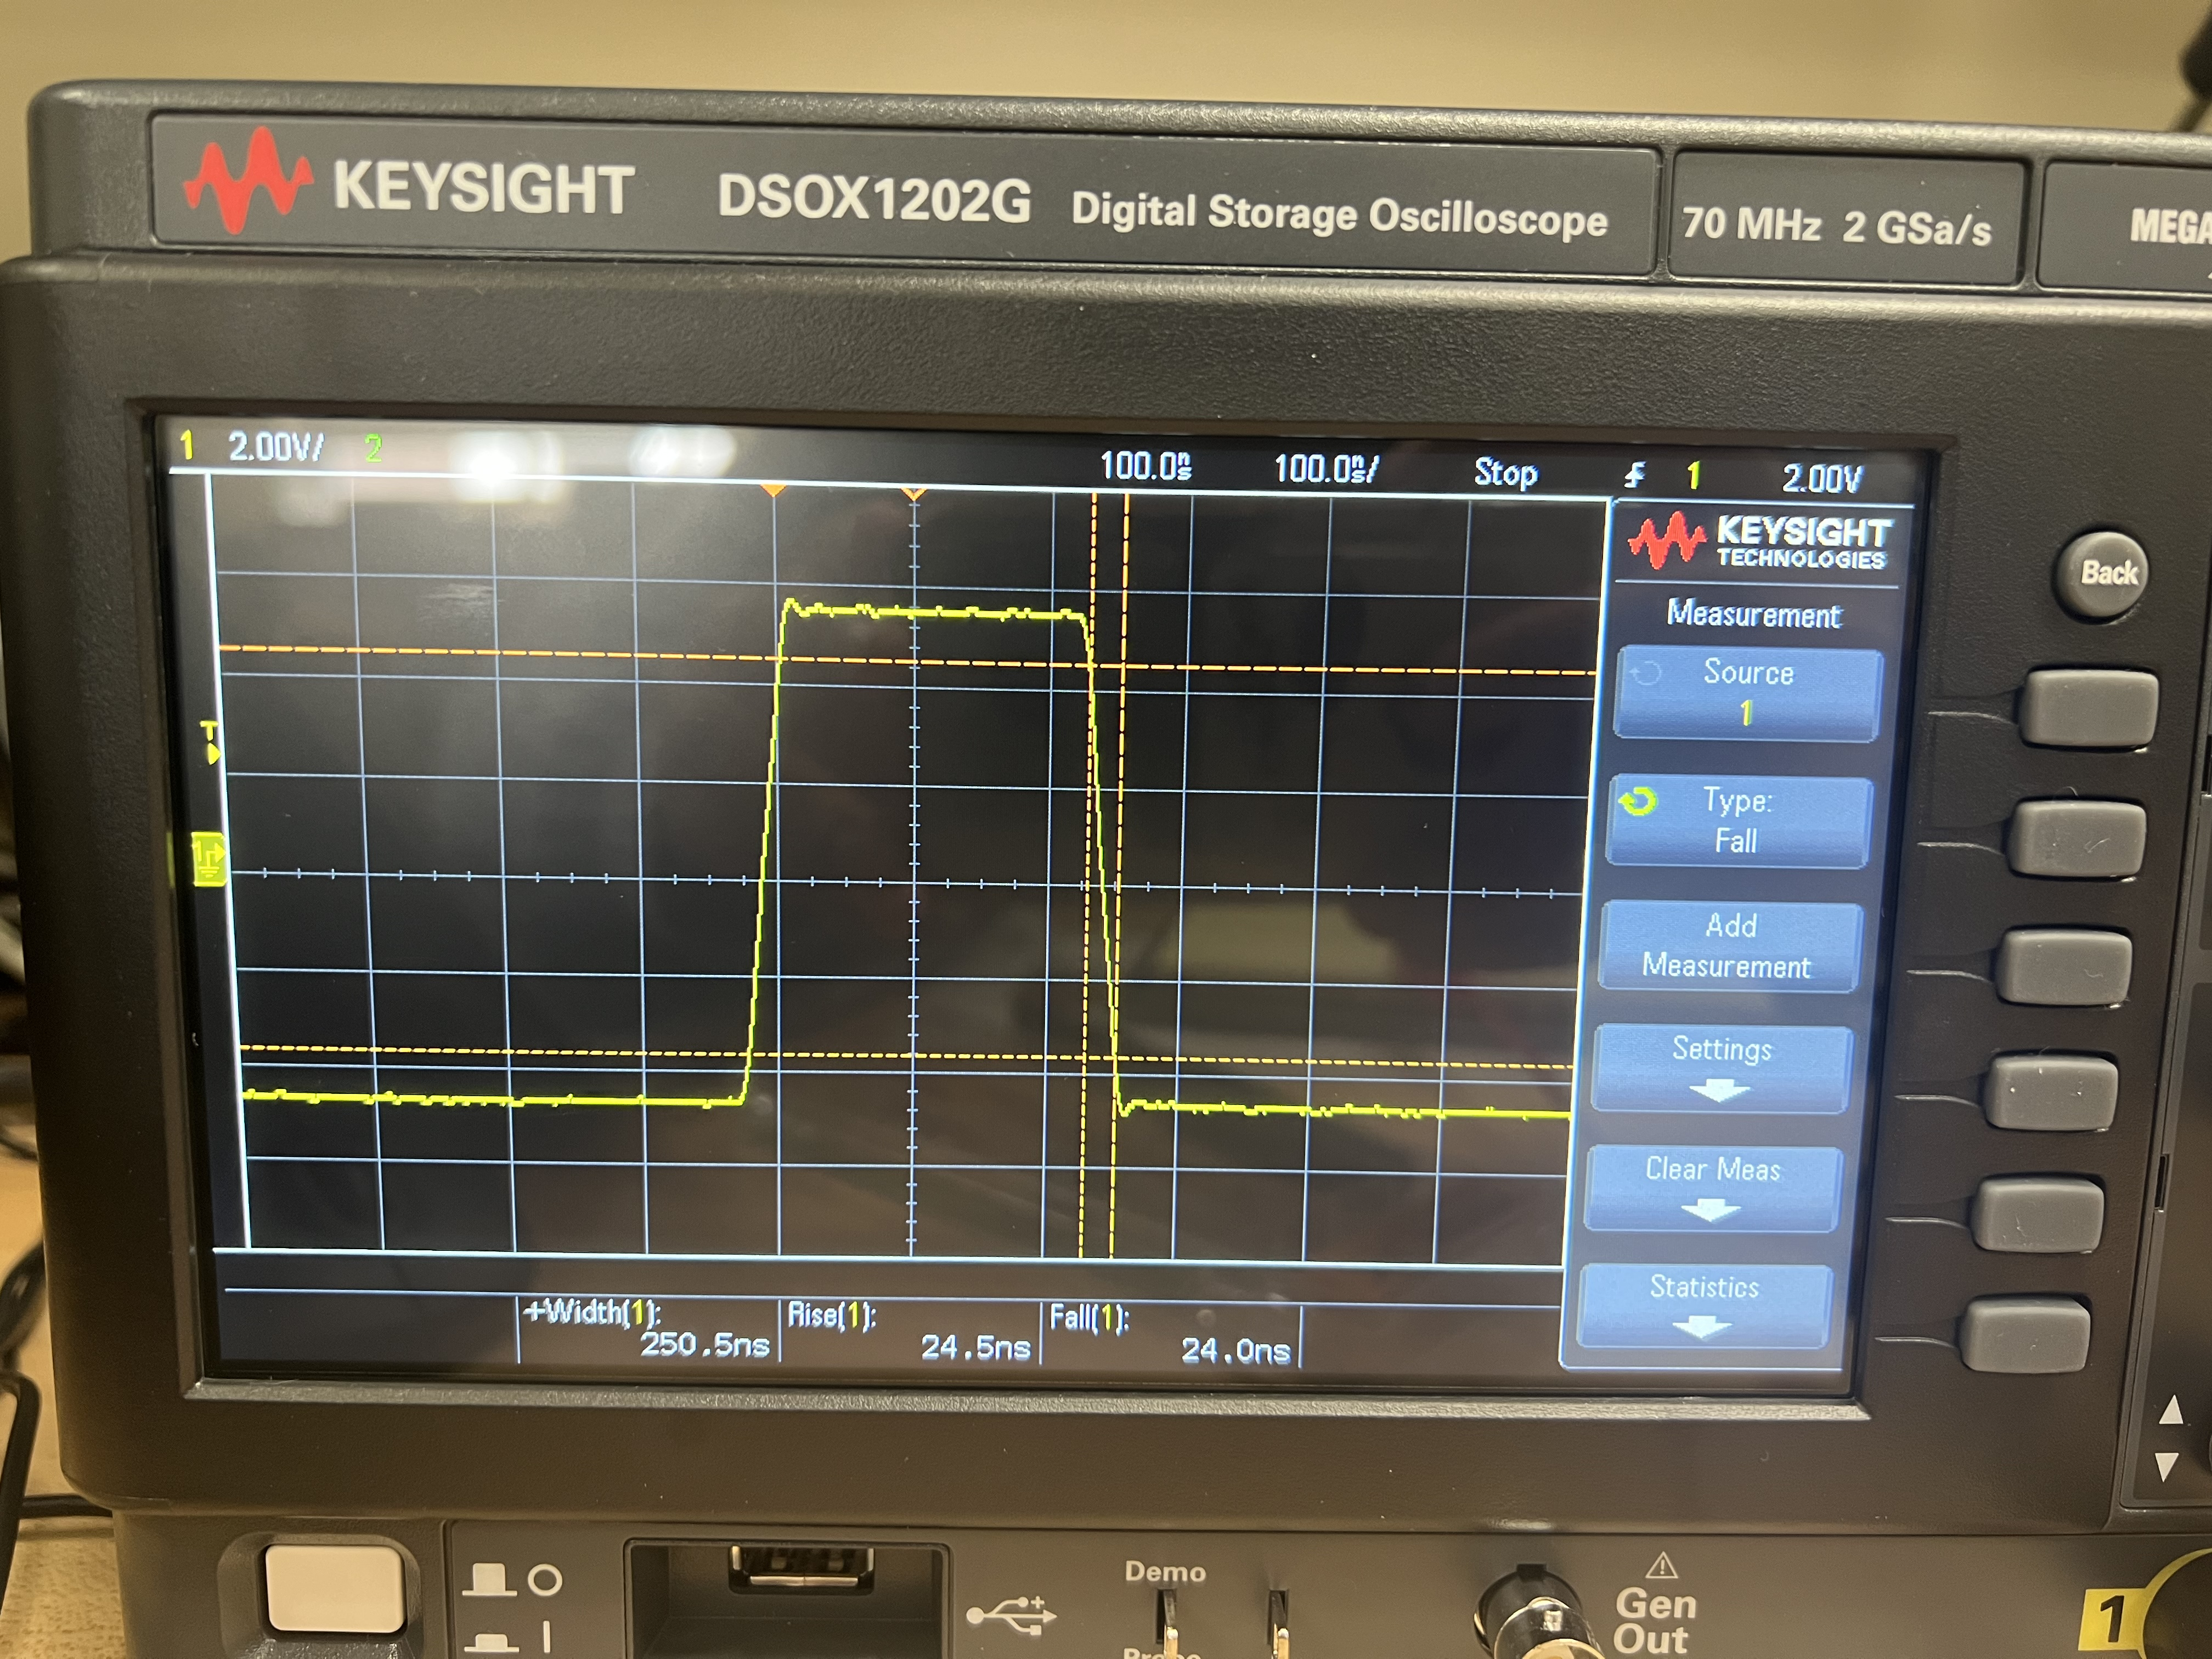
\includegraphics[width=0.5\textwidth]{PulseWaveform.jpeg}
    \caption{Pulse Waveform}
    \label{fig:Pulse-Waveform}
\end{figure}

\subsubsection{Sinusoidal Waveform}
\begin{enumerate}
\setcounter{enumi}{2}
\item \textbf{Capture the Oscilloscope screen for a 10 ms interval} and save it to document your laboratory experiments.
\end{enumerate}
\begin{figure}[h]
    \centering
    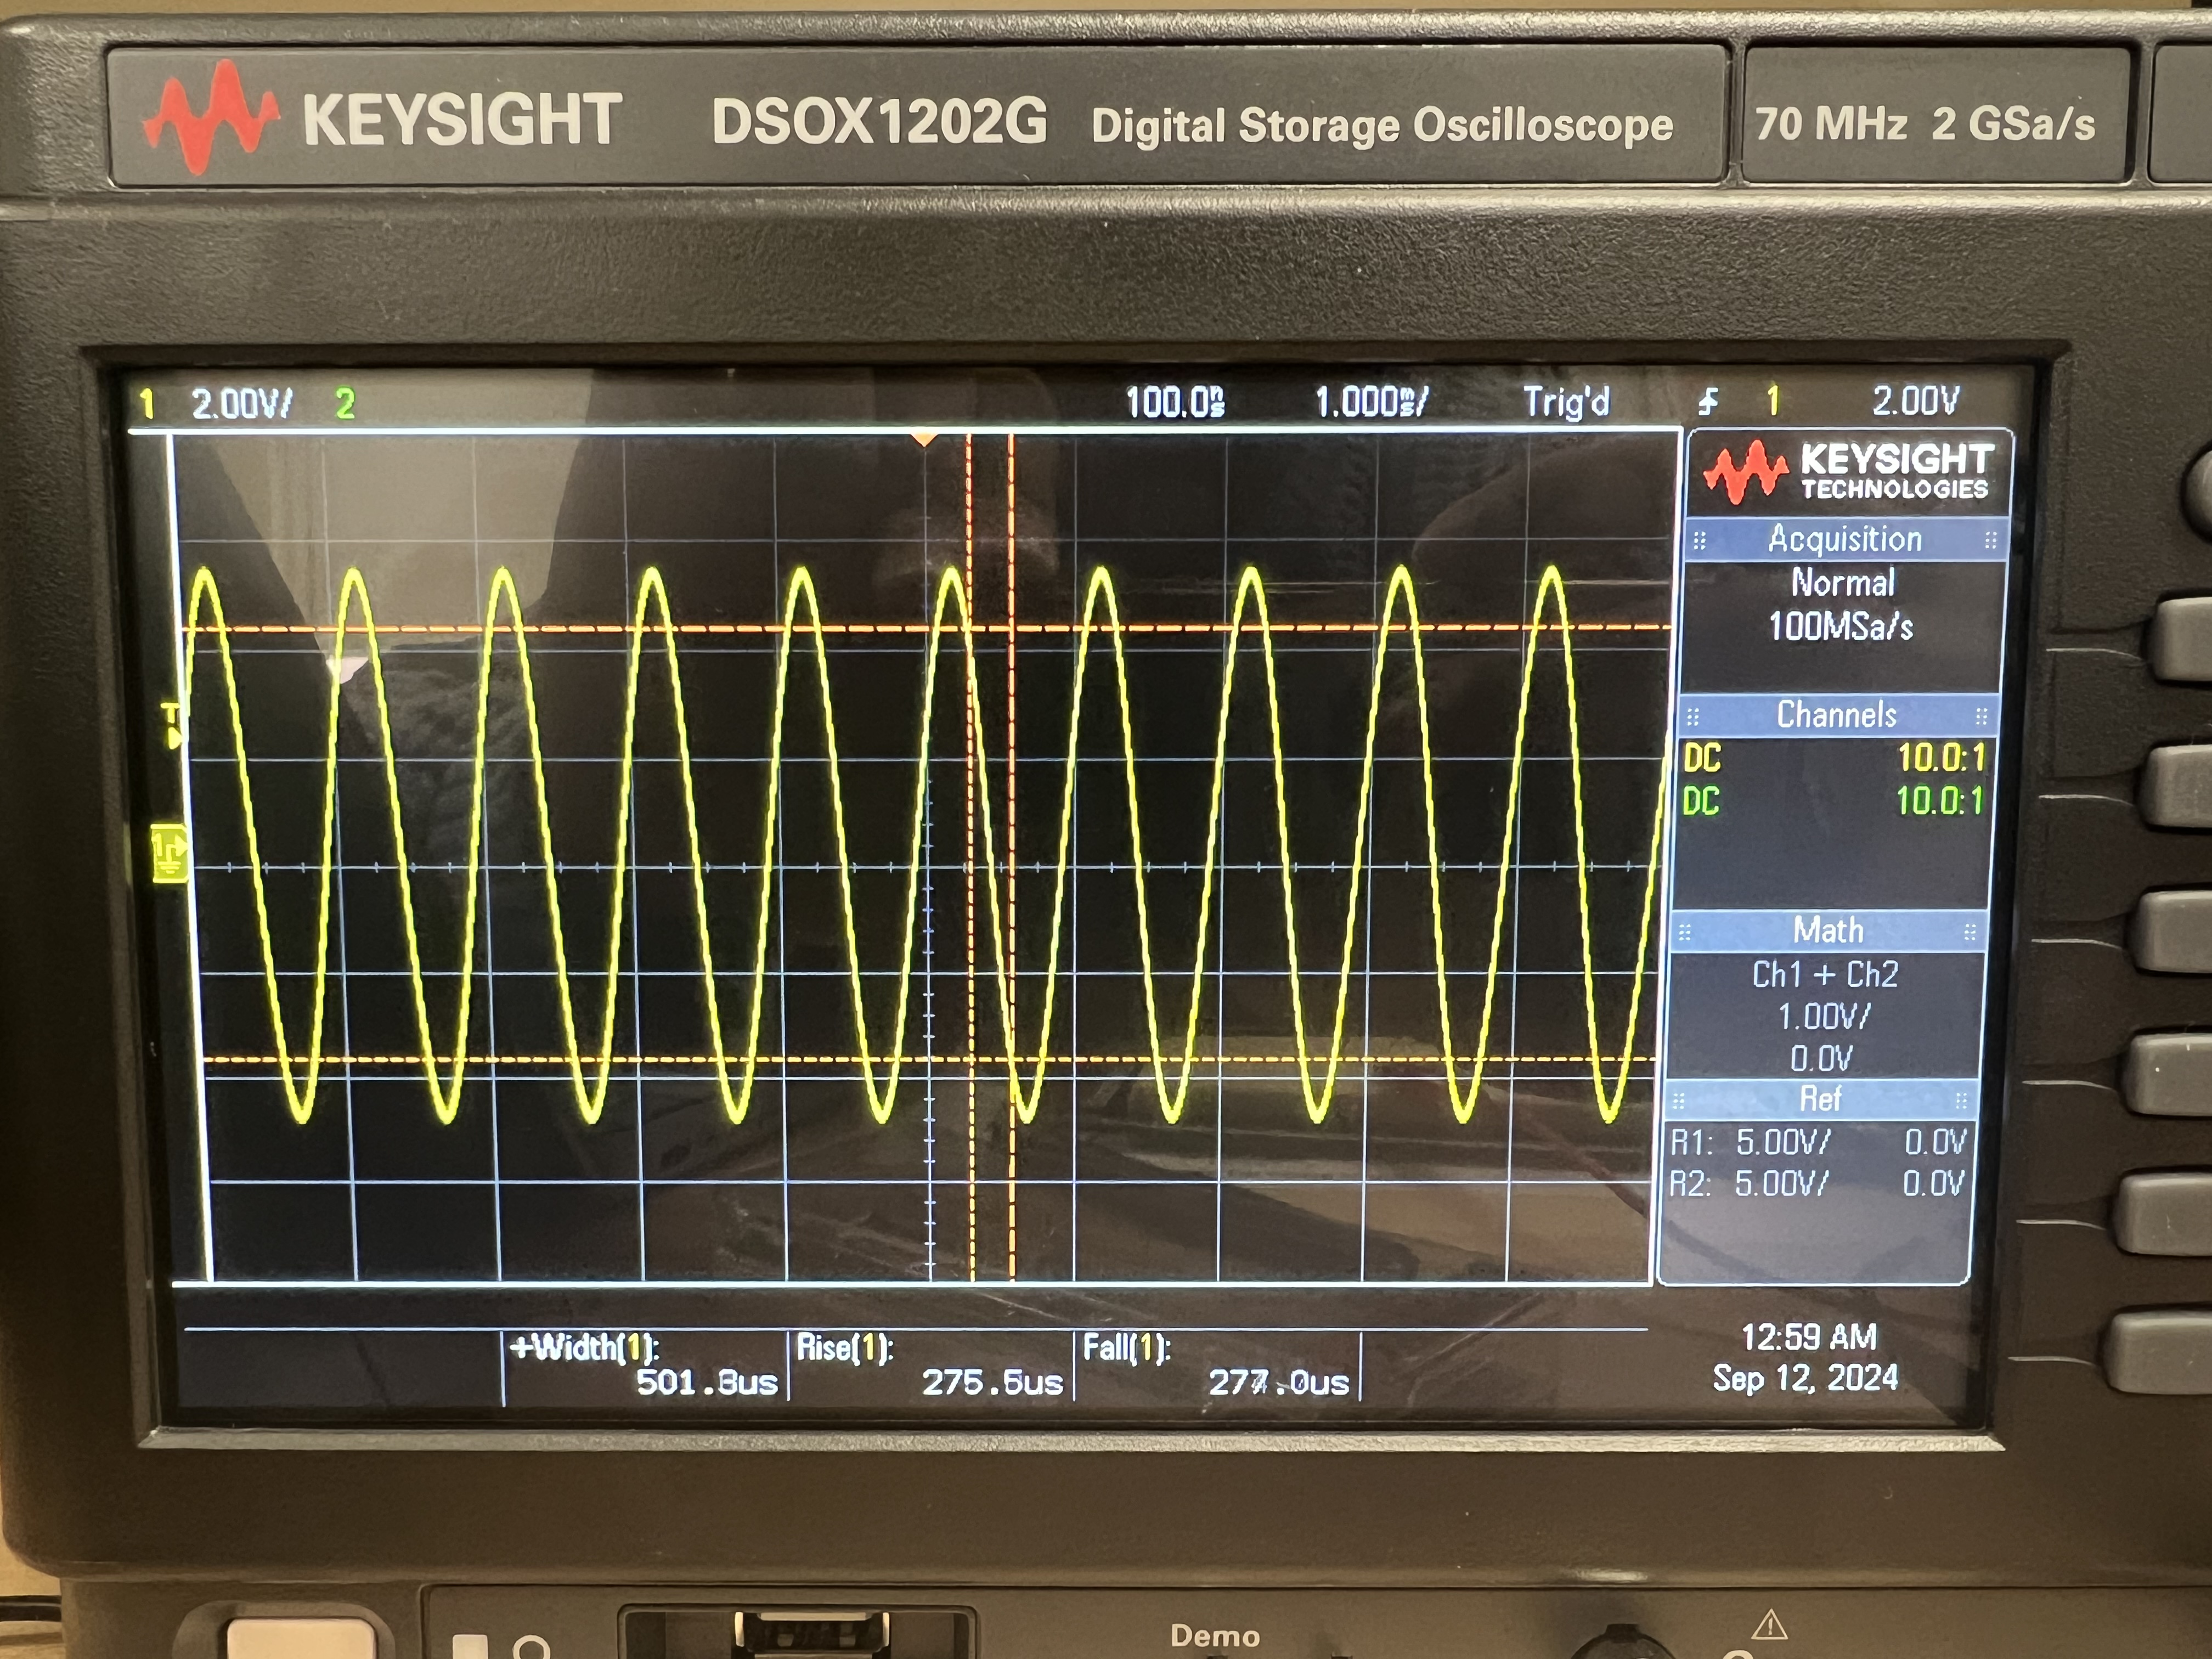
\includegraphics[width=0.6\textwidth]{SineWaveform.jpeg}
    \caption{Sinusoidal Waveform}
    \label{fig:Sinusoidal-Waveform}
\end{figure}

\subsubsection{Square Waveform}
\begin{enumerate}
\setcounter{enumi}{2}
\item \textbf{Capture the Oscilloscope screen for a 500 ms interval} and save it to document your laboratory experiments.
\end{enumerate}
\begin{figure}[h]
    \centering
    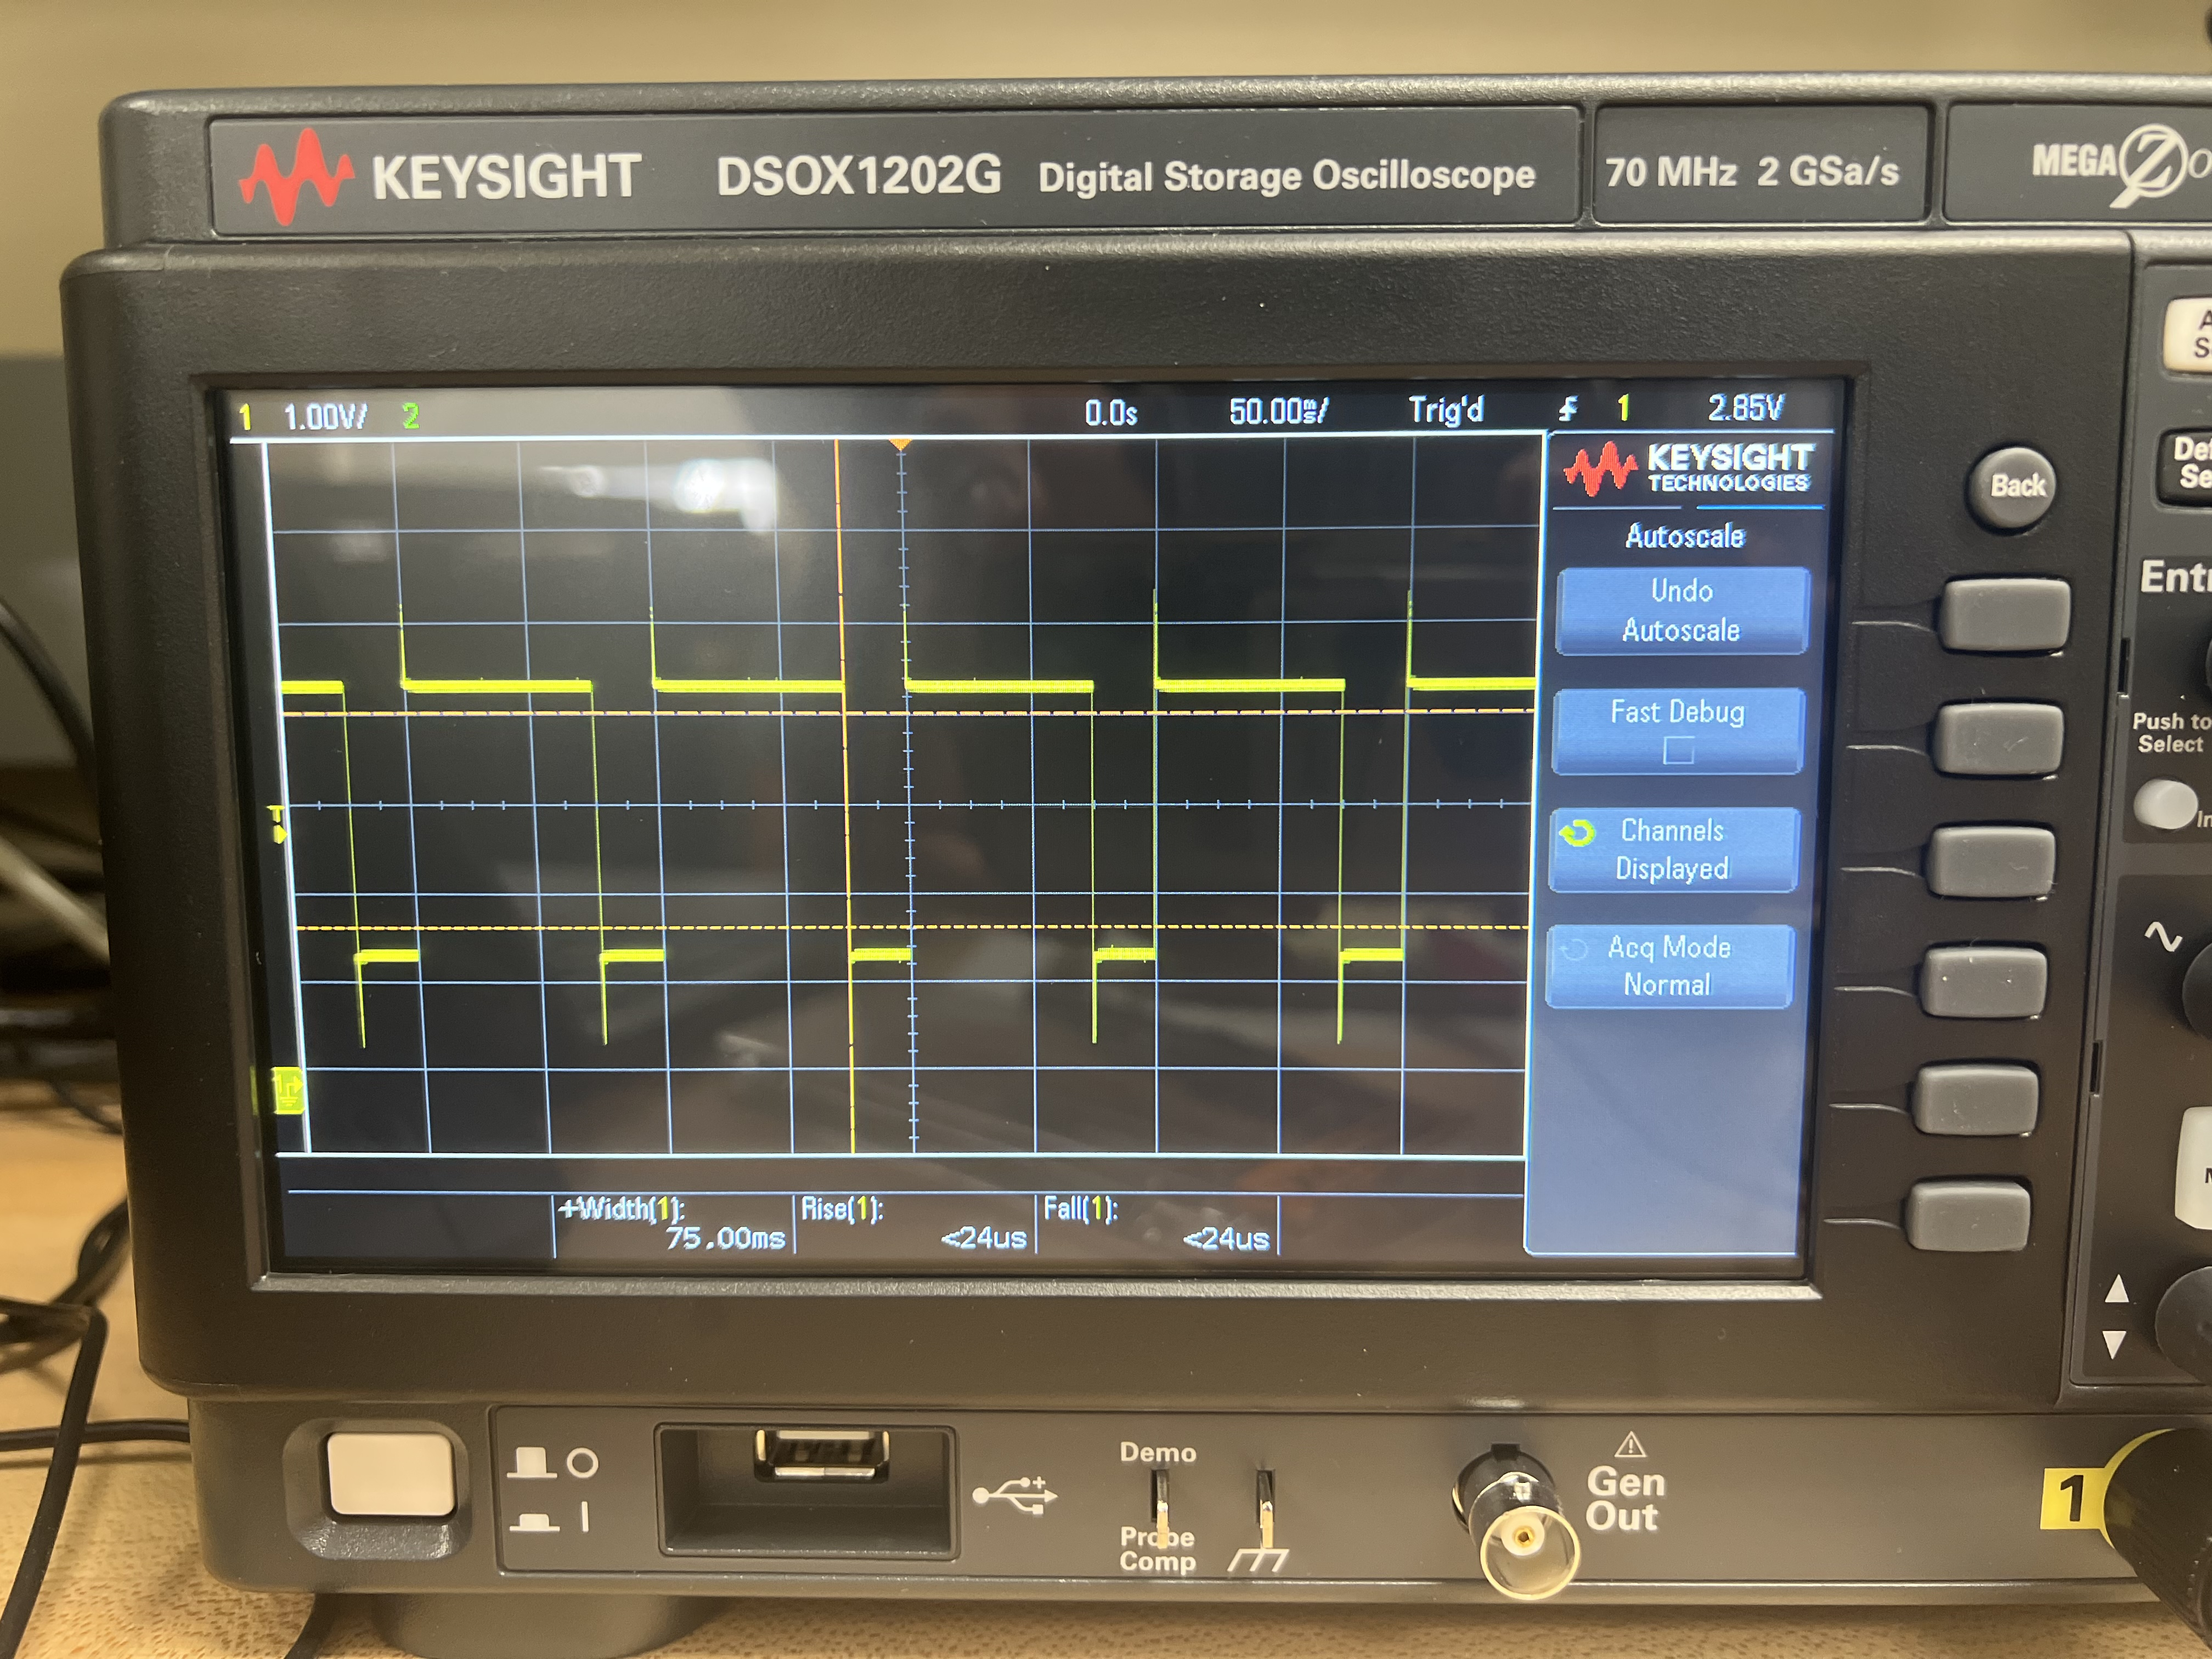
\includegraphics[width=0.6\textwidth]{SquareWaveform.jpeg}
    \caption{Square Waveform (noise approved by TA, Han)}
    \label{fig:Square-Waveform}
\end{figure}

\subsubsection{Triangle Waveform}
\begin{enumerate}
\setcounter{enumi}{2}
\item \textbf{Capture the Oscilloscope screen showing several cycles} and save it to document your laboratory experiments.
\end{enumerate}
\begin{figure}[h]
    \centering
    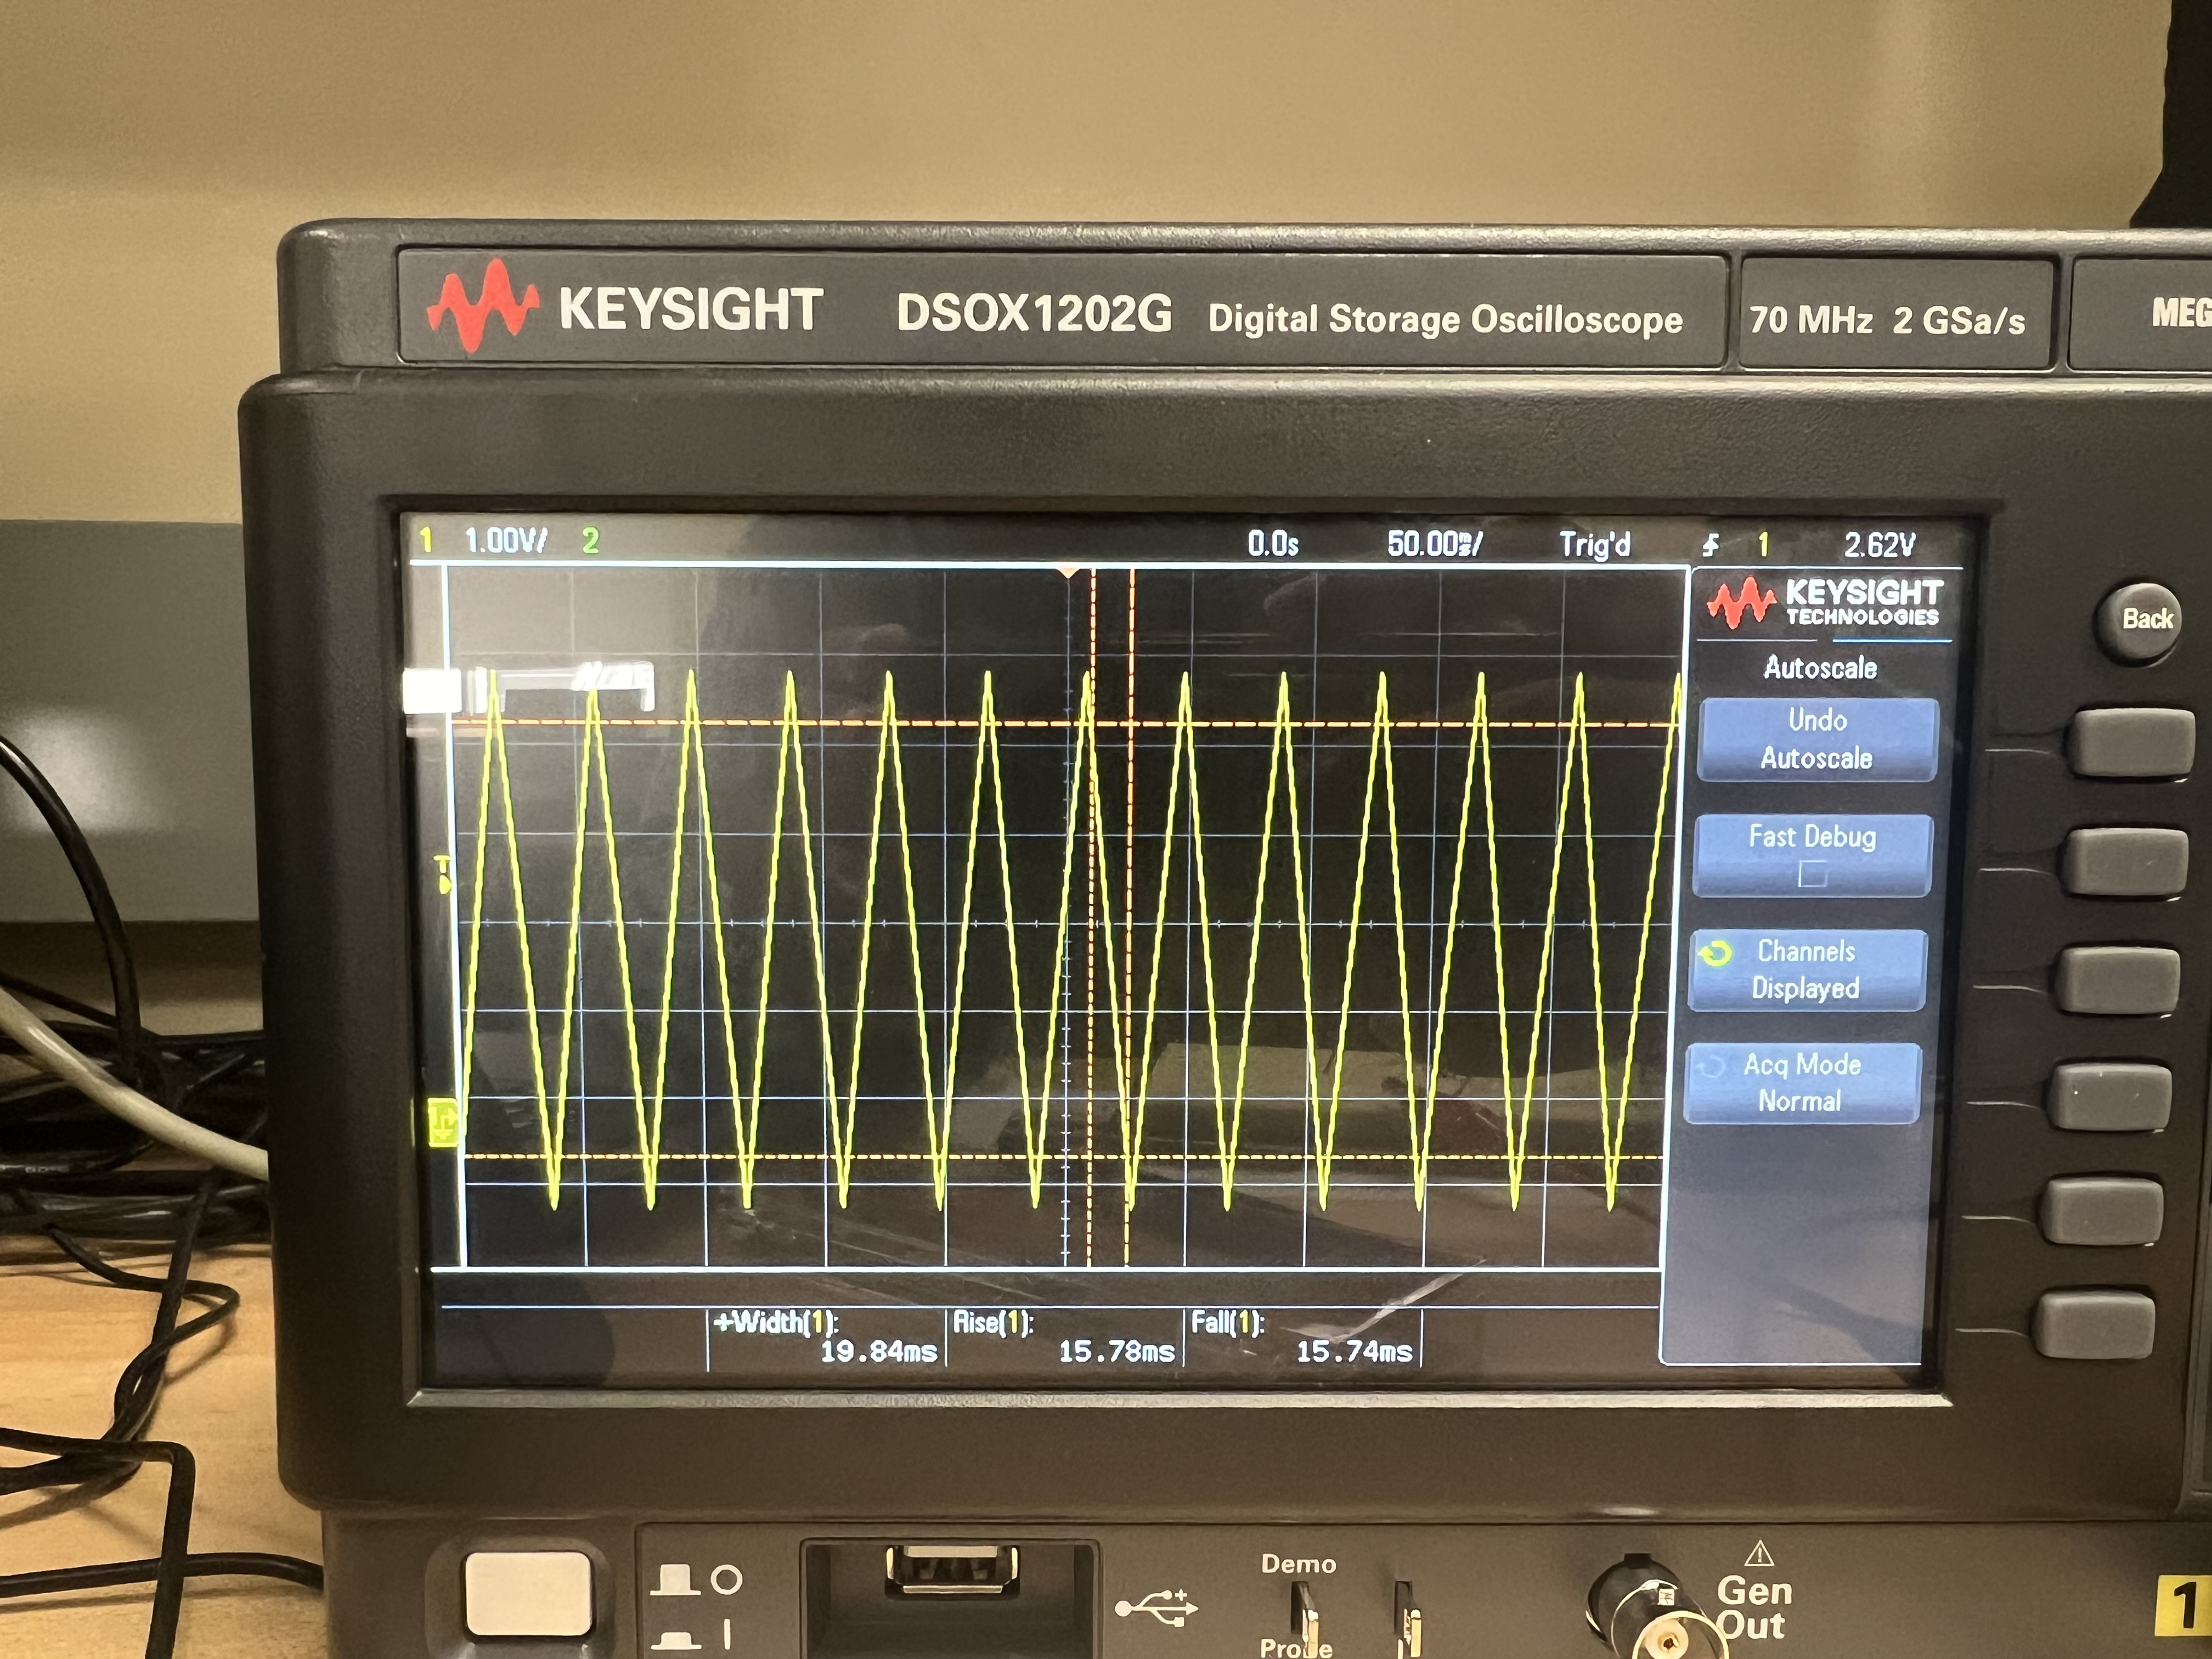
\includegraphics[width=0.6\textwidth]{TriangleWaveform.jpeg}
    \caption{Triangle Waveform}
    \label{fig:Triangle-Waveform}
\end{figure}


\section{Questions}
\begin{enumerate}
\item Define precision, accuracy, and resolution in your own words, and give an example of each.

Precision is how close your measurements are to each other. For example, measuring the same resistor multiple times and seeing how close all of your measured values were would provide a measure of precision.

Accuracy is how close your measurement is to the true value. For example, measuring a resistor and comparing it to the true value would provide a measure of accuracy.

Resolution is the smallest change in a quantity that can be detected by a measurement device. For example, if a multimeter provides 1 decimal point during measurement (ie 0.1V), it can detect changes of ± 0.05V.


\item Referencing your completed Table \ref{tab:Resolution}, why is the multimeter preferred for measuring voltage and current provided by the power supply as opposed to reading directly from the power supply display?

This is because the multimeter has a higher resolution than the power supply. 
The multimeter can measure voltage to the nearest 0.00005 mV, 
while the power supply can only measure to the nearest 0.0005 V. 
This means that the multimeter can provide a more accurate measurement of the voltage and current provided by the power supply.
Therefore, assuming no hardware faults, we can get more accurate measurements from the multimeter than from the power supply display.

\item Look up the internal resistances for both the voltmeter and ammeter capabilities for the Keysight 34461A Digital Multimeter used in lab. How do these values compare to the internal resistances you measured in section \ref{sec:measurements}? Give percent errors. \textit{Note: You can find the the input resistance for the voltmeter in the datasheet. Assume the input resistance for the ammeter is 2$\Omega$.}

Actual voltmeter resistance: 9.9355242 M$\Omega$ \\
Measured voltmeter resistance: 10 M$\Omega$ \\
Percent error $\approx \frac{10 - 9.9355242}{10} \times 100\% = 0.6448\%$

Actual ammeter resistance: 2.6913 $\Omega$ \\
Measured ammeter resistance: 2 $\Omega$ \\
Percent error $\approx \frac{2 - 2.6913}{2} \times 100\% = 34.565\%$

\item Suppose you want to produce a sinusoidal waveform with 5 V peak-to-peak voltage across a 25 $\Omega$ load using the function generator. When you do so, what will be the peak-to-peak voltage actually displayed on the front panel of the function generator and why? (Assume that the function generator has a standard internal 50 $\Omega$ resistance.)

$5 = V_{in} \cdot \frac{25}{25 + 50} = V_{in} \cdot \frac{25}{75} \implies V_{in} = 15 V$

Therefore, the input voltage to the function generator must be 15 V to produce a 5 V peak-to-peak voltage across a 25 $\Omega$ load. 
This is because of voltage division.

\end{enumerate}

\section{Extension}

\textit{When would a compensated oscilloscope probe be necessary when measuring timevarying waveforms? Give extreme cases and explain how an undercompensated and
overcompensated probe would adversely affect the measurement.}

A compensated oscilloscope probe is a type of probe that balances the probe's capacitance with the oscilloscope's input capacitance to prevent signal distortion, ensuring accurate measurements of high-frequency or time-varying waveforms.
Essentially it matches the capacitances to prevent any unecessary creation of filters and distortion of the signal.

A compensated oscilloscope probe is needed when measuring time-varying waveforms, particularly in circuits with high-frequency signals. Without compensation, the probe will distort waveform, while an overcompensated probe can cause overshoot, where the signal oscillates around its intended value. These distortions lead to inaccurate measurements, and so this is very important for sensitive measurements.

\end{document}
